% !TEX program = xelatex
% !TEX encoding = UTF-8 Unicode
\documentclass[12pt,a4paper,oneside]{report}
\makeatletter
\renewcommand\normalsize{%
  \@setfontsize\normalsize{13pt}{15.6pt}%
  \abovedisplayskip 12pt plus3pt minus7pt
  \belowdisplayskip \abovedisplayskip
  \abovedisplayshortskip 0pt plus3pt
  \belowdisplayshortskip 6.5pt plus3.5pt minus3pt}
\normalsize
\makeatother

\newcommand{\truong}{TRƯỜNG ĐẠI HỌC CÔNG NGHỆ THÔNG TIN VÀ TRUYỀN THÔNG}
\newcommand{\khoa}{KHOA CÔNG NGHỆ THÔNG TIN}
\newcommand{\loaibaocao}{BÁO CÁO TIỂU LUẬN}
\newcommand{\hocphan}{Học máy}
\newcommand{\lophocphan}{CNTT K22H + CNTT K22G}
\newcommand{\hocky}{Học kỳ 1, năm học 2026--2027}
\newcommand{\tendetai}{DỰ ĐOÁN XU HƯỚNG TĂNG/GIẢM GIÁ CỔ PHIẾU}
\newcommand{\tenbaitoan}{dự đoán xu hướng giá cổ phiếu}
\newcommand{\giangvien}{TS. Nguyễn Tuấn Anh}
\newcommand{\nhom}{Nhóm 16}
\newcommand{\svAten}{Trần Văn Hiếu}
\newcommand{\svAma}{DTC235200278}
\newcommand{\svBten}{Hoàng Đức Toàn}
\newcommand{\svBma}{DTC235200752}
\newcommand{\diadiem}{Thái Nguyên}
\newcommand{\thoigian}{tháng 12 năm 2026}

\usepackage[a4paper,left=3cm,right=2cm,top=2.5cm,bottom=2.5cm,
            headheight=16pt,headsep=0.8cm]{geometry}
\usepackage{fontspec}
\setmainfont{Times New Roman}
\IfFontExistsTF{Consolas}{\setmonofont{Consolas}[Scale=0.9]}{\setmonofont{Menlo}[Scale=0.85]}
\usepackage[vietnamese]{babel}
\usepackage{setspace}
\setstretch{1.3}
\setlength{\parindent}{1cm}
\setlength{\emergencystretch}{2em}
\setlength{\parskip}{6pt}
\usepackage{indentfirst}

\usepackage{amsmath,amssymb}
\usepackage{graphicx}
\graphicspath{{images/}}
\usepackage{float}
\usepackage{array,booktabs,tabularx,multirow,longtable}
\renewcommand{\arraystretch}{1.25}
\usepackage[table]{xcolor}
\usepackage{tikz}
\usetikzlibrary{positioning,arrows.meta,calc,fit,backgrounds}
\usepackage{caption}
\captionsetup{labelsep=period,labelfont=bf,font=normalsize,skip=6pt}
\captionsetup[table]{position=top}
\usepackage{titlesec}
\usepackage{titletoc}
\usepackage[nottoc]{tocbibind}
\usepackage{enumitem}
\setlist{nosep,leftmargin=1.6cm}
\usepackage{listings}
\usepackage{needspace}
\usepackage{cite}
\usepackage{fancyhdr}
\usepackage[unicode]{hyperref}
\hypersetup{
  hidelinks,
  pdftitle={\tendetai},
  pdfauthor={\svAten, \svBten},
  pdfsubject={\loaibaocao\ học phần \hocphan},
  bookmarksnumbered=true,
  bookmarksopen=true,
  bookmarksopenlevel=0,
}
\newcommand{\bmchapname}{Chương}
\makeatletter
\newcommand*{\bm@prefix}{}
\let\bm@orig@writebookmark\Hy@writebookmark
\renewcommand*{\Hy@writebookmark}[5]{%
  \ifnum#4=0 \def\bm@prefix{\bmchapname\space}\else\def\bm@prefix{}\fi
  \bm@orig@writebookmark{#1}{#2}{#3}{#4}{#5}}
\renewcommand*{\Hy@numberline}[1]{\bm@prefix#1. }
\makeatother

\definecolor{codebg}{RGB}{247,247,247}
\definecolor{codekw}{RGB}{0,51,153}
\definecolor{codecm}{RGB}{0,128,0}
\definecolor{codestr}{RGB}{163,21,21}
\definecolor{guide}{RGB}{110,110,110}
\lstdefinestyle{python}{
  language=Python,
  basicstyle=\ttfamily\small\setstretch{1.0},
  backgroundcolor=\color{codebg},
  keywordstyle=\color{codekw}\bfseries,
  commentstyle=\color{codecm}\itshape,
  stringstyle=\color{codestr},
  numbers=left, numberstyle=\tiny\color{guide}, numbersep=8pt,
  frame=single, rulecolor=\color{black!25},
  breaklines=true, showstringspaces=false, tabsize=4,
  xleftmargin=1.2em, framexleftmargin=1.2em,
  aboveskip=8pt, belowskip=8pt, columns=fullflexible, keepspaces=true,
}
\lstset{style=python}
\renewcommand{\lstlistingname}{Đoạn mã}
\renewcommand{\lstlistlistingname}{DANH MỤC ĐOẠN MÃ}

\addto\captionsvietnamese{%
  \renewcommand{\contentsname}{MỤC LỤC}%
  \renewcommand{\listfigurename}{DANH MỤC HÌNH ẢNH}%
  \renewcommand{\listtablename}{DANH MỤC BẢNG}%
  \renewcommand{\bibname}{TÀI LIỆU THAM KHẢO}%
  \renewcommand{\figurename}{Hình}%
  \renewcommand{\tablename}{Bảng}%
  \renewcommand{\chaptername}{Chương}%
  \renewcommand{\appendixname}{Phụ lục}%
}

\pagestyle{fancy}
\fancyhf{}
\fancyhead[L]{\small\itshape Báo cáo tiểu luận học phần \hocphan}
\fancyhead[R]{\small\itshape\nouppercase{\leftmark}}
\fancyfoot[C]{\thepage}
\renewcommand{\headrulewidth}{0.4pt}
\renewcommand{\chaptermark}[1]{\markboth{\chaptertitlename~\thechapter. #1}{}}
\fancypagestyle{plain}{\fancyhf{}\fancyfoot[C]{\thepage}\renewcommand{\headrulewidth}{0pt}}

\titleformat{\chapter}[display]
  {\filcenter\bfseries\fontsize{14}{18}\selectfont}
  {\MakeUppercase{\chaptertitlename}~\thechapter}{4pt}{\MakeUppercase}
\titlespacing*{\chapter}{0pt}{0pt}{18pt}
\titleformat{\section}
  {\bfseries\fontsize{14}{18}\selectfont}{\thesection.}{0.5em}{}
\titlespacing*{\section}{0pt}{12pt}{6pt}
\titleformat{\subsection}
  {\bfseries\fontsize{13}{17}\selectfont}{\thesubsection.}{0.5em}{}
\titlespacing*{\subsection}{0pt}{10pt}{6pt}
\setcounter{secnumdepth}{3}
\titleformat{\subsubsection}
  {\bfseries\itshape\fontsize{13}{17}\selectfont}{\thesubsubsection.}{0.5em}{}
\titlespacing*{\subsubsection}{0pt}{8pt}{4pt}

\setcounter{tocdepth}{2}
\newcommand{\tocchapname}{Chương}
\titlecontents{chapter}[0pt]{\addvspace{6pt}\bfseries}
  {\tocchapname~\thecontentslabel.\enspace}{}{\titlerule*[0.6pc]{.}\contentspage}
\titlecontents{section}[1.5em]{}
  {\thecontentslabel.\enspace}{}{\titlerule*[0.6pc]{.}\contentspage}
\titlecontents{subsection}[3em]{}
  {\thecontentslabel.\enspace}{}{\titlerule*[0.6pc]{.}\contentspage}
\titlecontents{figure}[0pt]{}
  {\figurename~\thecontentslabel.\enspace}{}{\titlerule*[0.6pc]{.}\contentspage}
\titlecontents{table}[0pt]{}
  {\tablename~\thecontentslabel.\enspace}{}{\titlerule*[0.6pc]{.}\contentspage}

\newcommand{\unnumberedchapter}[1]{%
  \chapter*{#1}\phantomsection\addcontentsline{toc}{chapter}{#1}\markboth{#1}{}}
\newcommand{\huongdan}[1]{{\color{guide}\itshape [Hướng dẫn: #1]}}
\newcommand{\khunghinh}[3]{%
  \begin{tikzpicture}
    \draw[dashed,thick,black!40,fill=black!3] (0,0) rectangle (#1,#2);
    \node[text width=0.8*#1,align=center,font=\itshape\color{guide}]
      at ($(0,0)!0.5!(#1,#2)$) {#3};
  \end{tikzpicture}}
\newcommand{\dongcham}[1]{\par\noindent\foreach \i in {1,...,#1}{\makebox[\linewidth]{\dotfill}\\[4pt]}}


\begin{document}
\pagestyle{plain}

\unnumberedchapter{NHẬT KÝ ĐÓNG GÓP}

Nhóm quản lý mã nguồn và báo cáo trong một kho Git chung. Mỗi thành viên commit bằng tài khoản của chính mình nên lịch sử commit là minh chứng cho phần đóng góp của từng người. Mục này gồm ảnh chụp lịch sử commit, bảng thống kê và nhật ký công việc theo tuần.

\section*{1. Lịch sử commit}

\begin{figure}[H]
  \centering
  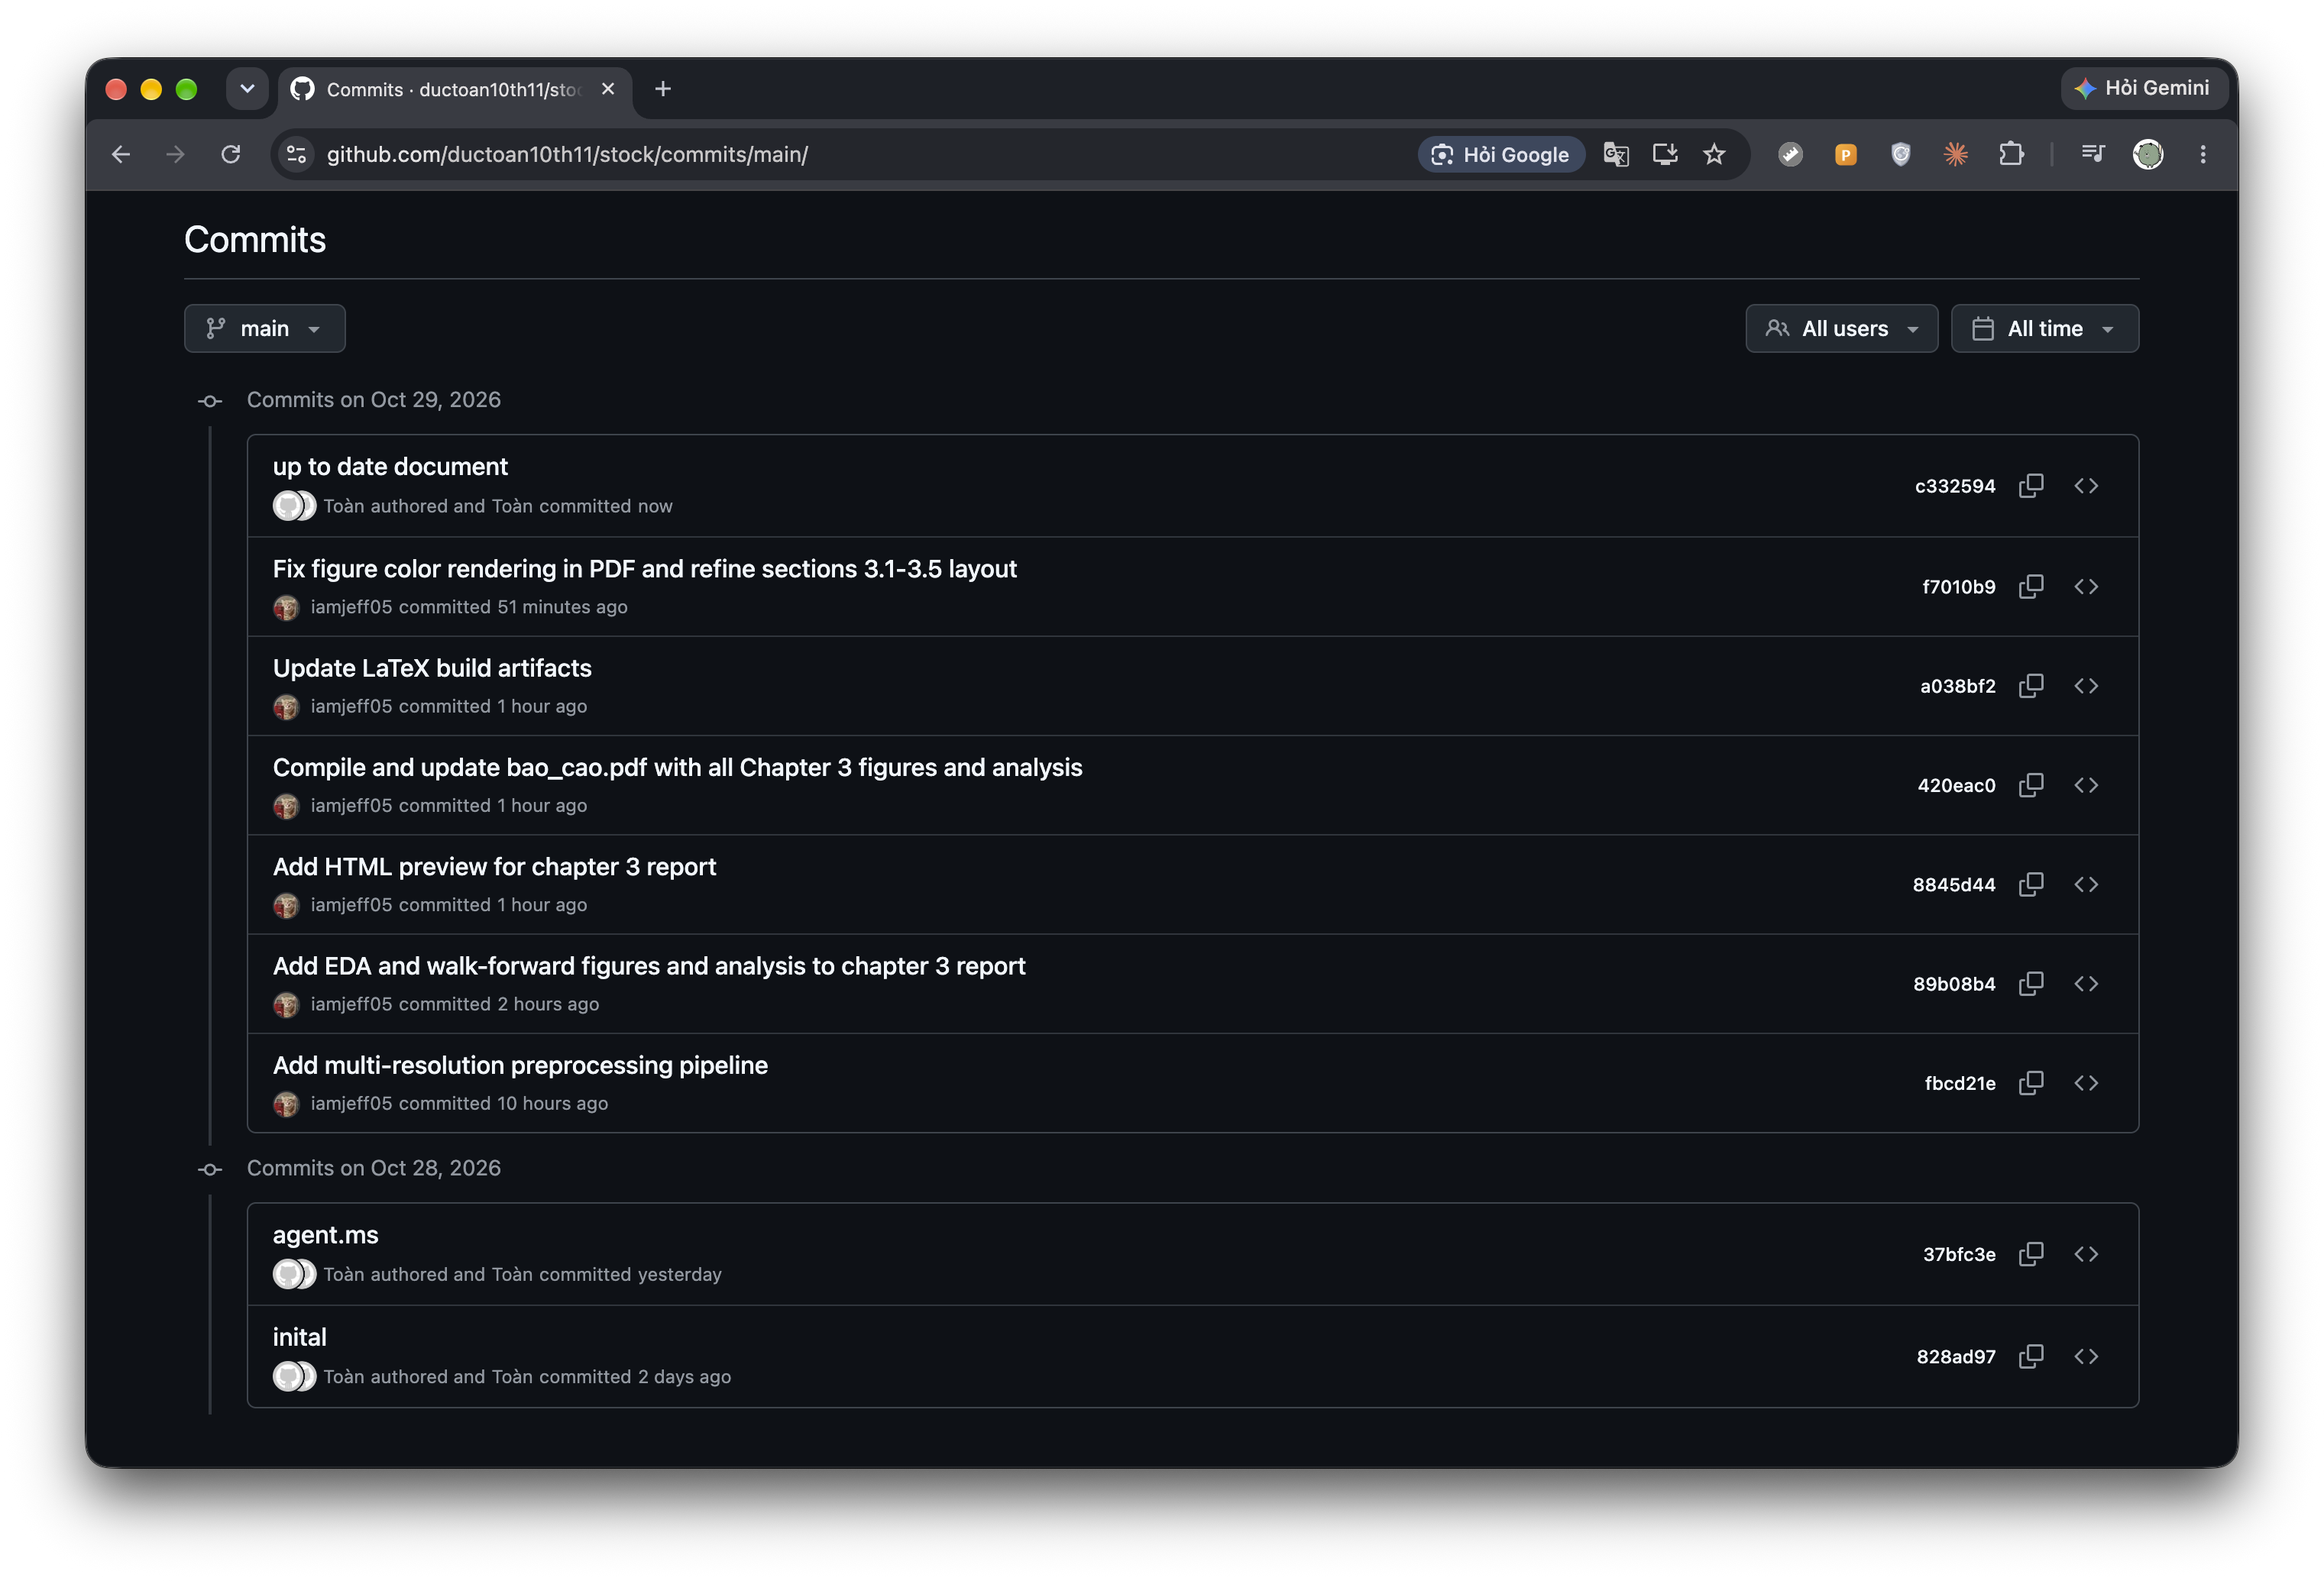
\includegraphics[width=\textwidth]{commit.png}
  \caption{Lịch sử commit của nhóm trên kho mã nguồn}
  \label{fig:commit-history}
\end{figure}

\section*{2. Thống kê theo thành viên}

\begin{table}[H]
  \centering
  \caption{Số commit của từng thành viên}
  \label{tab:commit-count}
  \begin{tabularx}{\textwidth}{p{4cm} >{\centering\arraybackslash}p{2.6cm} X}
    \toprule
    \textbf{Thành viên} & \textbf{Số commit} & \textbf{Nội dung chính} \\
    \midrule
    \svAten & 6 & Pipeline tiền xử lý, hình EDA và walk-forward, nội dung và bản dịch PDF của chương 3 \\
    \svBten & 3 & Khởi tạo kho, thu thập dữ liệu thô, tài liệu hướng dẫn cho agent, tách và cập nhật phần phân công và nhật ký đóng góp trong báo cáo \\
    \bottomrule
  \end{tabularx}
\end{table}

Số commit chỉ phản ánh một phần khối lượng công việc: một số commit chỉ cập nhật tệp sinh ra khi biên dịch LaTeX, trong khi các công việc như thiết kế tiền xử lý hay trao đổi thống nhất phương pháp không để lại commit riêng.

\section*{3. Chi tiết các commit}

\begin{table}[H]
  \centering
  \caption{Danh sách commit theo thời gian}
  \label{tab:commit-list}
  \small\begin{tabularx}{\textwidth}{p{1.9cm} p{1.6cm} p{2.7cm} >{\raggedright\arraybackslash}X}
    \toprule
    \textbf{Ngày} & \textbf{Mã} & \textbf{Thành viên} & \textbf{Nội dung} \\
    \midrule
    28/10/2026 & \texttt{828ad97} & \svBten & Khởi tạo kho; \texttt{crawl.py} và dữ liệu thô của 4 mã ở 6 khung nến \\
    28/10/2026 & \texttt{37bfc3e} & \svBten & Thêm \texttt{AGENTS.md}: quy ước làm việc và chống rò rỉ dữ liệu \\
    29/10/2026 & \texttt{fbcd21e} & \svAten & Thêm pipeline tiền xử lý đa khung: \texttt{clean\_data.py}, \texttt{preprocess\_data.py} \\
    29/10/2026 & \texttt{89b08b4} & \svAten & Thêm hình EDA, hình walk-forward và phần phân tích vào chương 3 \\
    29/10/2026 & \texttt{8845d44} & \svAten & Thêm bản xem trước HTML của chương 3 \\
    29/10/2026 & \texttt{420eac0} & \svAten & Biên dịch lại \texttt{bao\_cao.pdf} với đầy đủ hình chương 3 \\
    29/10/2026 & \texttt{a038bf2} & \svAten & Cập nhật tệp sinh ra khi biên dịch LaTeX \\
    29/10/2026 & \texttt{f7010b9} & \svAten & Sửa lỗi màu hình trong PDF, chỉnh bố cục các mục 3.1--3.5 \\
    29/10/2026 & \texttt{c332594} & \svBten & Cập nhật báo cáo: tách \texttt{phan-cong.tex}, \texttt{dong-gop.tex} và \texttt{preamble.tex}, thêm ảnh lịch sử commit, biên dịch lại PDF \\
    \bottomrule
  \end{tabularx}
\end{table}

\section*{4. Nhật ký công việc theo tuần}

\begin{table}[H]
  \centering
  \caption{Nhật ký công việc theo tuần}
  \label{tab:nhatky}
  \begin{tabularx}{\textwidth}{>{\centering\arraybackslash}p{1.4cm} >{\centering\arraybackslash}p{2.4cm} p{3.2cm} X}
    \toprule
    \textbf{Tuần} & \textbf{Ngày} & \textbf{Thành viên} & \textbf{Công việc / commit} \\
    \midrule
    1 & 23/10/2026 & \svBten & Thu thập dữ liệu nến của 4 mã bằng \texttt{crawl.py} \\
    1 & \dots & \svAten & Soạn báo cáo tuần 1 (Mở đầu, Chương 2, Chương 3) \\
    2 & 29/10/2026 & \svAten & Làm sạch 6 khung nến; tạo 25--30 đặc trưng và nhãn ba lớp cho toàn bộ 6 khung; cập nhật báo cáo \\
    \dots & \dots & \dots & \dots \\
    \bottomrule
  \end{tabularx}
\end{table}

\end{document}
